%%This is a very basic article template.
%%There is just one section and two subsections.
\documentclass{main}
 

\usepackage{graphicx}      % include this line if your document contains figures
\usepackage{natbib}        % required for bibliography
\usepackage{subfigure}
\usepackage{enumerate}


\begin{document}

\begin{frontmatter}

\title{THE EMBEDDED ELECTRONICS AND SOFTWARE OF ROSA ROBOT
\thanksref{footnoteinfo}} 

\thanks[footnoteinfo]{This work is supported by ESBR under contract COPPETEC
JIRAU 151/13 6631-0002/2013 (ANEL R\&D program).}

\author[1]{Renan S. Freitas}
\author[1]{Eduardo Elael M. S.}
\author[1]{Gabriel S. Alcantara}
\author[2]{Julia R. Campana}
\author[1]{Alessandro J. Peixoto}
\author[1]{Ramon R. Costa}
\author[3]{Sylvain Joyeux}
\author[3]{Patrick Paranhos}

  \address[1]{Electrical
 Engineering Department, COPPE UFRJ, Rio de Janeiro, Brazil}
  \address[2]{Professional and Technical Communication, Illinois Institute of
  Technology, Illinois, United States} 
  \address[3]{Research Department Robotics Innovation Center, German Research
 Centre for Artificial Intelligence (DFKI), Bremen, Germany}
 
\begin{abstract}                % Abstract of not more than 250 words.
ROSA is a research project which endeavors to design and implement a robot for
the monitoring and inspection tasks of the inserting and removing stoplogs
process in a power plant. The proposed system is mounted on the lifting beam,
which carries the stoplogs, and it is composed of different sensors:
inclination, pressure, and inductive sensors for monitoring; and a profiling
sonar with pan \& tilt system for inspection. This paper presents a general
overview of the robot, and a description of the developed embedded electronics, power supply system,
and software architecture. The field experiments at UHE Jirau, in Rond{\^o}nia,
Brazil, using a tablet for user interface validate the concepts considered so far.
\end{abstract}  

\begin{keyword}
field robotics; embedded electronics; robotic software architecture; sonar;
\end{keyword}

\end{frontmatter}

\section{Introduction}
Hydropower is the most mature, reliable and cost-effective
renewable power generation technology available \citep{brown}, accouting 16
percent of global electricity generation. The global hydropower use and
capacity will increase about 3.1\% each year for the next 25 years \citep{wi}.
The total investment for large-scale hydropower projects
typically range from USD 1000/kW to around USD 3500/kW and, once commissioned,
the annual operation and maintenance costs of hydropower plants are often
quoted as 4\% of the investment per kW per year \citep{ecofys}. 

In the specific case of Brazil, the third biggest hydroelectric potential of
the world, hydropower represents 84\% of its electric power total production.
Brazil is the second biggest country of installed hydropower capacity, 84 GW,
and in the Amazon basin, in Madeira river, this number will be increased next
years by the construction of Santo Antonio (3150 MW) and Jirau (3300 MW) power
plants. The dependance on this renewable power source mobilizes private
initiative investments on research centers and universities, and motivates the
development systems with a high degree of automation based on advanced robotic
systems \citep{aneel}.

A major challenge for hydropower companies is River water level
control for dam construction, flooding prevention, and the station
maintenance. Stoplogs are hydraulic engineering control elements that are used
as a solution for water level control. Several power plants use this technology, such as:
the Santa Clara River, in California, USA; the River Great Ouse, in King's Lynn, England; the
Lakefield Generating Station, in Lakefield, Canada; the Killaloe Canal, in
Ireland; the Goolwa Barrage, in Australia; and UHE Jirau, in Rond{\^o}nia,
Brazil. Figure~\ref{figs:intro:goolwa} illustrates the stoplog installation in
Goolwa Barrage.

\begin{figure}[ht]
\centering
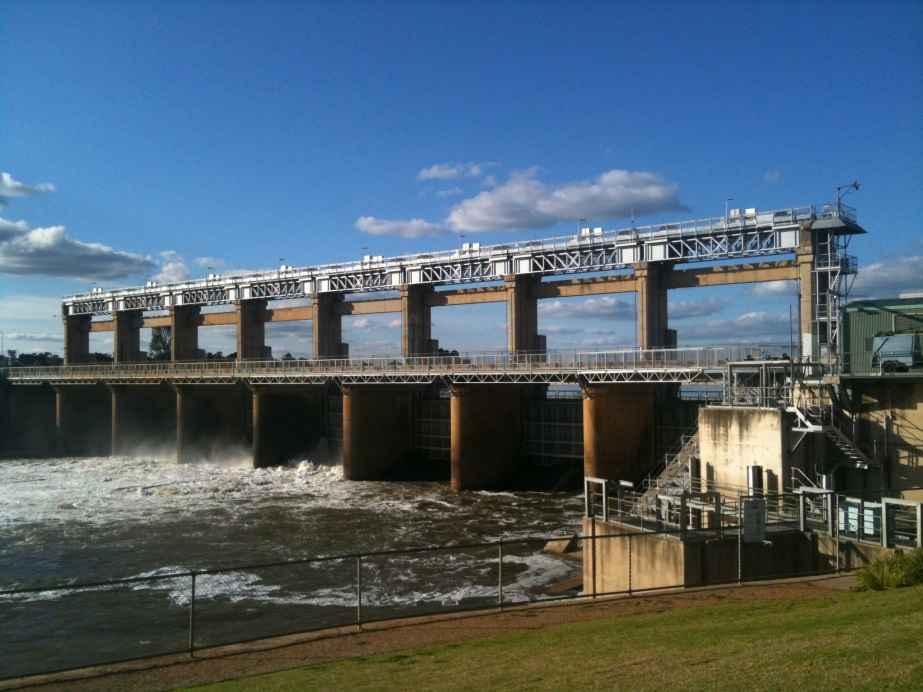
\includegraphics[width=8.4cm]{figs/intro/goolwa.jpg}
\caption{The Goolwa barrage}
\label{figs:intro:goolwa}
\end{figure}

Stoplogs are modular and manually operated. At inserting or removing process,
the operator of a gated structure controls the water
level in channel by adding or removing individual stoplogs with a lifiting beam.
However, problems may occur during the process: bad coupling between lifting
beam and stoplog, bad stoplog stacking due to sediments, and difficult removal
owing to silt particles accumulation and hydrostatic pressure. In the specific
case of Jirau power plant, in Rond{\^o}nia, Brazil, the Madeira River tears out
trees along the stretch, carrying more than 500 tons of sediments every day
\citep{amazon}.

\citet{jack} studies stoplogs and lifting beam's physical and
mechanical properties. The ideal stoplog, as mentioned in the book, has a
mechanical contact sensor, and an hydrostatic pressure regulator valve, which
solve most of the problems on stoplog operations. However, in \cite{pinc},
England, a technical standard is proposed for
manufacturing, cost and maintenance reasons, and without the sensing technology.
Regarding solving stoplog installation issues, increasing efficiency and
reducing downtime, companies develop robotic systems. Besides, robots can replace humans in tasks
performed in unhealthy and hazardous areas, improving Health,
Safety, and Environment (HSE) conditions.

The Ontario Ministry of Natural Resources (OMNR) operates the Ivanhoe Lake Dam,
in Ontario, Canada, to regulate water levels with stoplogs for flooding
prevention of the downstream community of Foleyet. The dam's
configuration posed a risk to the operators: the deck is two meters above the
top stoplog and the operators needed to
manually grapple it from deck level using a hook on the end of
a pike pole, often forced to reach and feel for the log several feet inder
waterm being exposed to hazardous conditions, high water and high flow-speed
conditions. In 2006, Hatch, an engineering and development consultancy,
developed a system composed of a lifting beam with submersible proximity sensors
and submersible electric servomotors to independently actuate the hook. In 2007,
the system was installed at Ivanhoe Lake Dam greatly improving safety by
reducing the amount of manual handling required in this hazardous environment
\citep{hatch}.

Similarly, the Atlas Polar log lifter automates the process of stoplog
installation. The system is composed of an inductive sensor
recessed in the compactor plate to sense contact with the log and a force
sensor, stain gauge, which will indicate stoplog release or lifting
\citep{atlas}.


In this paper, we present a general overview of the ROSA robot, and a detailed
description of the embedded electronics, power supply system and software
architecture. The robot is designed to perform monitoring and inspection
tasks of the stoplogs' stacking and retrieving process in a power
plant. Carrying different sensors, the robot analyses sensor data \emph{in
loco} or stores it for a posterior analysis, interprets the results, and
sends specific data to the operator. The sensors can identify the lifting beam
actual operation (stack/retrieve), stoplog attachment/detachment, the
lifting beam inclination, the system depth in water, and the system has a
profiling sonar for sediments inspection. 

This text is organized as follows: a general overview of the robot and its main
challenges are presented in Section \ref{sec:general_overview}, detailed
descriptions of the embedded electronics, the vehicle support system, power
supply system, and software architecture are taken in
Sections \ref{sec:electronics_overview}, \ref{sec:powersupply_overview}, and
\ref{sec:software} respectively.
In Section \ref{sec:results}, preliminary results are shown, and concluding
remarks are drawn in Section \ref{sec:conclusions}.
\section{General Overview}\label{sec:general_overview}
\section{Embedded Electronics}\label{sec:electronics_overview}
\section{Power Supply System}\label{sec:powersupply_overview}
\section{Software Architecture}\label{sec:software}
\section{Experimental tests and results}\label{sec:results}
\section{Conclusions and future work}\label{sec:conclusions}
  
\bibliography{main} 
\appendix
\end{document}
